\section{Callbacks}
Javascript ist eine auf Events basierende Programmiersprache. Das bedeutet, anstatt auf blockierenden Code zu warten, führt Javascript Operationen weiter aus und reagiert wenn die Aktion fertig ist. Um sicherzustellen, dass Javascript auf die Fertigstellung von asynchronen Operationen wartet, wurden \textbf{Callbacks} eingeführt. Doch was genau sind Callbacks?

\subsection{Funktionale Programmierung}

Sowohl in Javascript als auch in Typescript sind Funktionen als Erste-Klasse-Objekte zu sehen. Aus diesem Grund ist es Möglich sie an Variablen, als Argumente in anderen Funktionen oder als Rückgabewert zu übergeben. Diese übergebenen Funktionen heißen Callbacks.\\

\noindent
Callbacks, auch Rückruffunktionen genannt, bildet das Kernkonzept der funktionalen Programmierung in Javascript.\cite{callbacks-intro} In der funktionalen Programmierung sind Funktionen als Werte zu betrachten. Der Code besteht aus kleineren Funktionen, die in höher geordneten Funktionen eingesetzt oder miteinander kombiniert werden können (Komposition). Dadurch ist der Code wiederverwendbar und weniger fehleranfällig. Javascript bietet mit Arrays die Möglichkeit Callbacks sinnvoll einzusetzen. Vor dem Ausführen des Beispiels muss folgend konfiguriert werden:

\begin{center}
    async-patterns$\,\to\,$ webpack.config.js
\end{center}

\begin{figure}[H]
\begin{lstlisting}[basicstyle=\small]
module.exports = {
    mode: 'development',
    entry: './src/modules/callbacks/introduction.ts',
    ...
}
\end{lstlisting}
\end{figure}

\begin{figure}[H]
\begin{lstlisting}[basicstyle=\small]
const numbers: number[] = [1, 2, 3, 4, 5, 6];
function isEven(x): boolean { 
  return x % 2 === 0; 
}

const evenNumbers = numbers.filter(isEven);
console.log(evenNumbers) // 2 4 6
\end{lstlisting}
\caption{Die Funktion filter() gibt ein neues Array zurück.}
\end{figure}

\noindent
Die Methode filter() nimmt Elemente einer Liste heraus, basierend einer Funktion die, die Filterkonditionen bestimmt. Dabei wird zuerst, dass Element aus der Liste entnommen und dann die Kondition geprüft. Da Funktionen als Argument anderer Funktionen übergeben werden, ist es Möglich diese \glqq{}später\grqq{} innerhalb des Funktionsrumpfes aufzurufen \textit{(Call back)}. Wenn also eine Funktion als Parameter übergeben wird, wird diese nicht sofort ausgeführt. Eine Funktion die ein Callback als Input-Parameter annimmt, wird auch High-Order-Funktion genannt.\cite{callbacks-example} Möchte man das Filtern klassisch implementieren, dann würde der Code im Vergleich dazu so aussehen:

\begin{figure}[H]
\begin{lstlisting}[basicstyle=\small]
const newArr = [];

for (let i = 0; i < numbers.length; i++) {
    if (numbers[i] % 2 === 0) {
        newArr.push(numbers[i]);
    }
}

console.log(newArr);
\end{lstlisting}
\end{figure}

\noindent
Wie man nun sehen kann, ist man mit dieser Umsetzung an externe Variablen gebunden. Diese könnte im Verlauf des Codes eventuell überschrieben werden. Das heißt der unten ausgeführte Code ist abhängig vom Status des Arrays. Dies führt zu einer erhöhten Fehleranfälligkeit. Wenn man nun alle ungeraden Zahlen herausfiltern möchte, müsste man ein neues Array mit einer neuen Schleife erstellen. In diesem Fall wird keine Möglichkeit der Wiederverwendbarkeit gewährleistet.

\subsection{Asynchrone Verarbeitung}
Ein Ansatz der asynchronen Verarbeitung ist die Nutzung von Funktionen die eine Funktion als Argument annehmen und erst dann diese Aufrufen, wenn eine blockierende Aktion fertig ausgeführt wurde. Dieses Verhalten ist nützlich wenn der Browser von bestimmten, zeitintensiven Aktionen abhängig ist. In den folgenden drei Kapitel (Callbacks, Promises und Async await) wird der gleiche Anwendungsfall, in drei verschiedenen Ansätzen angewendet und gegenübergestellt. Mit der REST-Api \textbf{JSONPlaceholder} wird ein Endpunkt für die Datenabfrage definiert. Hierbei handelt es sich um eine Open Source Endstelle die Beispieldaten für das Prototyping oder zum Testen zur Verfügung stellt. Je nach Anwendungsfall werden verschiedene Ausführungen von Anfragen an diese Endstelle geführt, um die Code-Beispiele so praxisnah wie Möglich zu halten.

\subsection{Beispiel}
Das folgende Code-Beispiel richtet sich nach dem funktionalen Programmierparadigma, da durch die Nutzungen von \textbf{puren Funktionen}, das Callback-Prinzip besser zur Geltung kommt. Eine pure Funktion, ist eine Funktion die beim selben Input jedes mal das gleiche Output wiedergibt. Für das Beispiel sollte folgend konfiguriert werden:

\begin{center}
    async-patterns$\,\to\,$ webpack.config.js
\end{center}

\begin{figure}[H]
\begin{lstlisting}[basicstyle=\small]
module.exports = {
    mode: 'development',
    entry: './src/modules/callbacks/stories.ts',
    ...
}
\end{lstlisting}
\end{figure}

\begin{figure}[H]
\begin{lstlisting}[basicstyle=\small]
function makeRequest(url, onSuccess, onFailure?): void {
    const req = new XMLHttpRequest();
    req.open('GET', url);

    req.onload = () => {
        if (req.status === 200) {
            fakeLatency(() => onSuccess(req.response));
        }
    };

    req.onerror = () => onFailure(Error('Network Error'));

    req.send();
}

function fakeLatency(callback): void {
    setTimeout(callback, 3000 * Math.random());
}
\end{lstlisting}
\end{figure}

\begin{figure}[H]
\begin{lstlisting}[basicstyle=\small]
function baseUrl(): string {
    return 'https://jsonplaceholder.typicode.com/posts/';
}

function createElm(innerHTML): HTMLElement {
    const div = document.createElement('div');
    div.innerHTML = innerHTML;
    document.body.appendChild(div);
    return div;
}

function getAllChapters(onSuccess, onFailure?): void {
    makeRequest(baseUrl(), onSuccess, onFailure);
}

function getChapter(chapter, onSuccess, onFailure?): void {
    makeRequest(baseUrl() + chapter.toString(), onSuccess, onFailure);
}

function spawn(content): void {
    content = JSON.parse(content);

    if (content instanceof Array === false) {
        content = [content];
    }

    content.forEach(elm => {
        const snippet = document.createElement('div');
        snippet.innerHTML = `<h1>${elm.title}</h1>
                           <div class="story-info">
                               <i>ID: Post-${elm.id}</i>
                           </div>
                           <p>${elm.body}.</p>`;

        document.body.insertBefore(snippet, loadingIcon);
    });
}
\end{lstlisting}
\end{figure}

\begin{figure}[H]
\begin{lstlisting}[basicstyle=\small]
function catchError(err) {
     createElm(`Ooops! Error Occurred! ${err}`);
}

function displayFinished(): void {
    loadingIcon.style.display = 'none';
    createElm('<div>All done!</div>');
}

const loadingIcon = createElm(`<svg>...</svg>`);
\end{lstlisting}
\end{figure}

\noindent
Dabei sind die wichtigsten Funktionen makeRequest(), getAllChapters(), getChapter() und spawn(). MakeRequest() führt eine Http-Anfrage gegen einen definierten Endpunkt aus. Wenn der Status der Antwort 200 beträgt, wird im Success-Callback vorangeschreitet. Bei einem Fehler wird der Error-Callback aufgerufen. Sowohl getAllChapter() als auch getChapter() führen makeRequest() aus mit der Möglichkeit im Erfolgs- und im Fehlerfall der Anfrage eine Aktion auszuführen. Spawn() nimmt ein Argument entgegen und lädt diesen in die HTML-DOM. Sollte ein Anwendungsfall sein, alle Kapitel der API anzufragen und bei Ankunft der Daten in die DOM zu laden, würde dies wie folgt aussehen:

\begin{figure}[H]
\begin{lstlisting}[basicstyle=\small]
getAllChapters(function(response) {
    spawn(response);
    displayFinished();
});
\end{lstlisting}
\end{figure}

\noindent
In diesem Fall wird spawn() erst aufgerufen, wenn eine Antwort vom Endpunkt ankommt. Um multiple asynchrone Operationen nacheinander auszuführen, müssen Funktionen ineinandergeschachtelt werden. So wird die Ausführung sequentiell fortgesetzt:

\begin{figure}[H]
\begin{lstlisting}[basicstyle=\small]
getChapter(1, function(response1) { // (*)
    spawn(response1);
    getChapter(2, function(response2) { // (**)
        spawn(response2);
        getChapter(3, function(response3) { // (***)
            spawn(response3);
            displayFinished();
        });
    });
});
\end{lstlisting}
\end{figure}

\noindent
Auffallend in diesem Beispiel wird der Grad an Einrückung, der mit jeder weiteren asynchronen Operationen steigt. Ein neuer Thread entsteht schon beim Aufruf von getChapter(1). Alle weiteren asynchronen Operationen sind voneinander abhängig und bleiben innerhalb des selben Zeitfensters. Asynchronität ist ansteckend. Eine Funktion, die zur asynchronen Verarbeitung ein Callback nutzt, operiert selbst asynchron. Wenn nun ein Großteil eines Programms aus ineinandergeschachtelten Funktionen besteht, kann diese Struktur zur erhöhten Fehleranfälligkeit führen. Dank der der sechsten Ecmascript-Version ist es auch Möglich Pfeil-Funktionen in Javascript zu nutzen. Diese sind syntaktisch kürzer als anonyme Funktionen. Bei der Verarbeitung des Fehlgeschlagenen Callbacks, würde der Code so aussehen:

\begin{figure}[H]
\begin{lstlisting}[basicstyle=\small]
getChapter(1, response1 => { // (*)
    spawn(response1);
    getChapter(2, response2 => { // (**)
        spawn(response2);
        getChapter(3, response3 => { // (***)
            spawn(response3);
            displayFinished();
        }, err3 => catchError(err3)); // (***)
    }, err2 => catchError(err2)); // (**)
}, err1 => catchError(err1)); // (*)
\end{lstlisting}
\caption{Es bildet sich ein sog. Baum, der sich immer weiter nach rechts ausbreitet.}
\end{figure}

\noindent
Zusammenfassend kann man also sagen, dass in dem synchronen Modell implizit auf die Aktionen gewartet wird, und in dem asynchronen Modell explizit. Als Diagramm abgebildet führt der Browser die Methoden wie folgt aus:

\begin{center}
\begin{figure}[H]
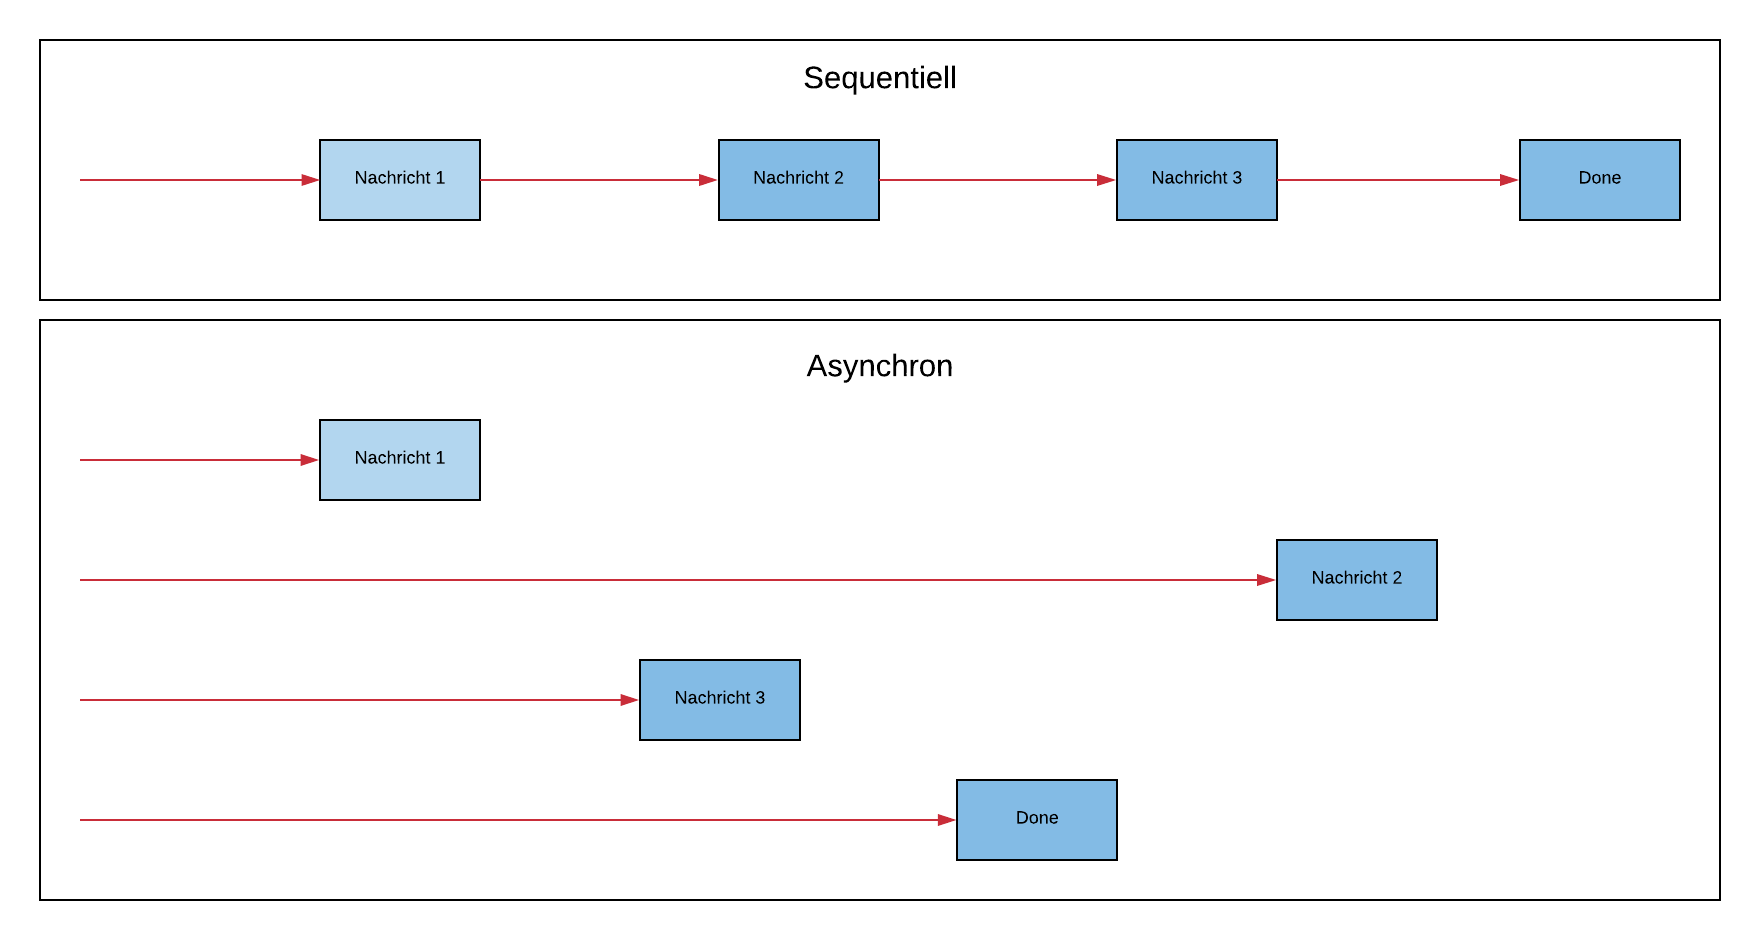
\includegraphics[width=12cm]{synchron-vs-asynchron-diagram}
\caption{Ablauf der ausgeführten Operationen im Browser}
\end{figure}
\end{center}

\noindent
Hier werden mehrere Level von Callback-Funktionen ineinander geschachtelt, um die Abhängigkeiten der Aufrufe zu wahren. Sollte jetzt bei einer selbsterstellten Callback-Funktion ein zusätzliches Error-Handling berücksichtigt werden, wird die Nachvollziehbarkeit einer höherrangigen Funktion kaum noch gewährleistet. Der Code oben wird deshalb auch als Callback-Hell bezeichnet.




